\label{sec:pieao_method}
Согласно сказанному в разделе \ref{sec:piezo_theor}, в определенных кристаллографических
направлениях при воздействии внешнего электрического поля, будет возникать деформация
сжатия или растяжения. Этим деформациям соответсвует изменение межплоскостного
 расстояния, которое может быть измерено с помощью дифракции рентгеновского
 излучения, а именно, по измерению углового сдвига дифракционного пика \cite{marchenkov2014}.
 %
 % \begin{figure}[H]
 %   \centering
 %   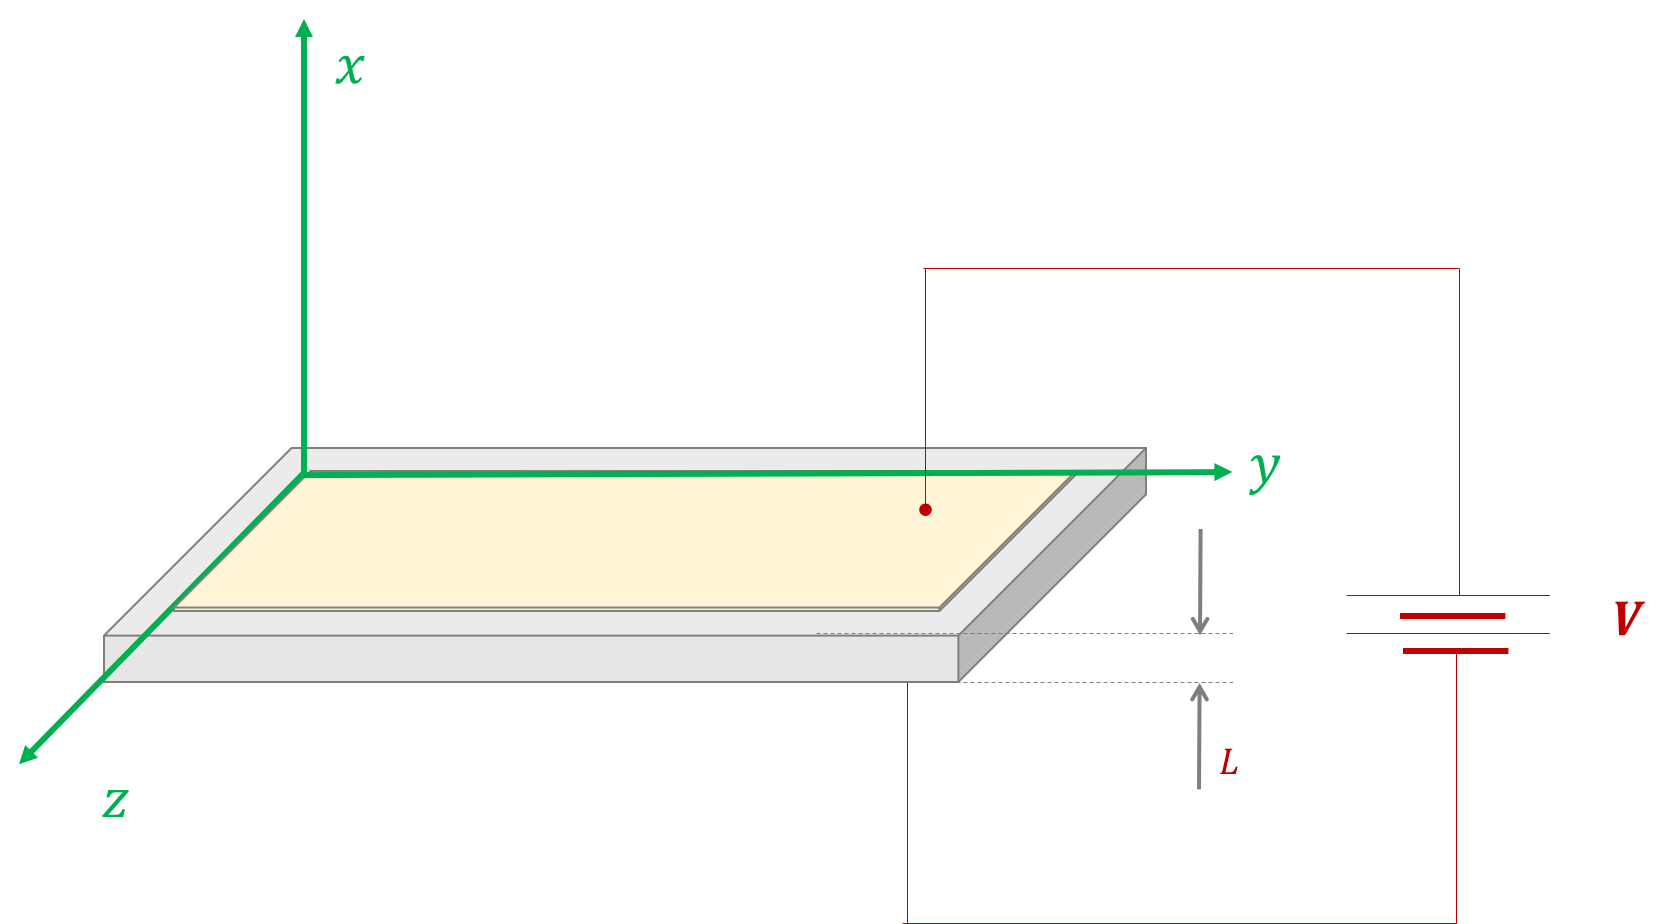
\includegraphics[width=.4\textwidth]{images/piezo.png}
 %   \caption{Приложенное электрическое поле к $x$ - срезу образца}
 %   \label{ris:x_cut}
 % \end{figure}

Исходя из закона Вульфа - Брэгга, если межплоскостное расстояние получило приращение
$\Delta d$, тогда:
$$ \Delta d = \frac{\lambda}{2}\left( \frac{1}{\sin(\theta_B + \Delta \theta) } - \frac{1}{\sin \theta_B } \right), $$
\noindent
а изменение угла отражения $\Delta \theta$ составит:
\begin{equation}
   \Delta \theta =-  \frac{\tan \theta_B}{\frac{d}{\Delta d}+1}  = -  \frac{\Delta d }{d}  \tan \theta_B,
\end{equation}
\noindent
где $\Delta d/d = r$ - относительное изменение межплоскостного расстояния.
Таким образом, учитывая связь с
(\ref{eq:piezomodule}),  в кристалле толщиной $L$ и разностью потенциалов на его
гранях $V$ напряженность электрического поля составляет $E = \frac{V}{L}$, а
относительная деформация, необходимая для вычисления пьезомодуля
 рассчитывается исходя из следующего выражения:
 \begin{equation}
    \frac{\Delta d}{d}  = -\frac{\Delta \theta \cdot L}{V \tan \theta_B}.
    \label{eq:piezomodule_l}
 \end{equation}

Выражение (\ref{eq:piezomodule_l}) было использовано в
\cite{kibalin2015, marchenkov2014,piezo101,piezo102} для
пересчета углового сдвига брэгговского максимума в величину пьезоэлектрического модуля.
Следует отметить, такой подход не является общим и имеет существенные ограничения при
измерении, например, сдвиговых пьезомодулей, а также в том случае, если параметр решетки
в направлении деформации определяется величиной более чем одного пьезомодуля $d_{ij}$.

На рис. \ref{ris:piezo_deformation_general} изображена триклинная элементарная ячейка
(в качестве общего случая),
а также обозначены кристаллографические направления по отношению к декартовой
системе координат.

\begin{figure}[H]
  \centering
  \subfloat[]{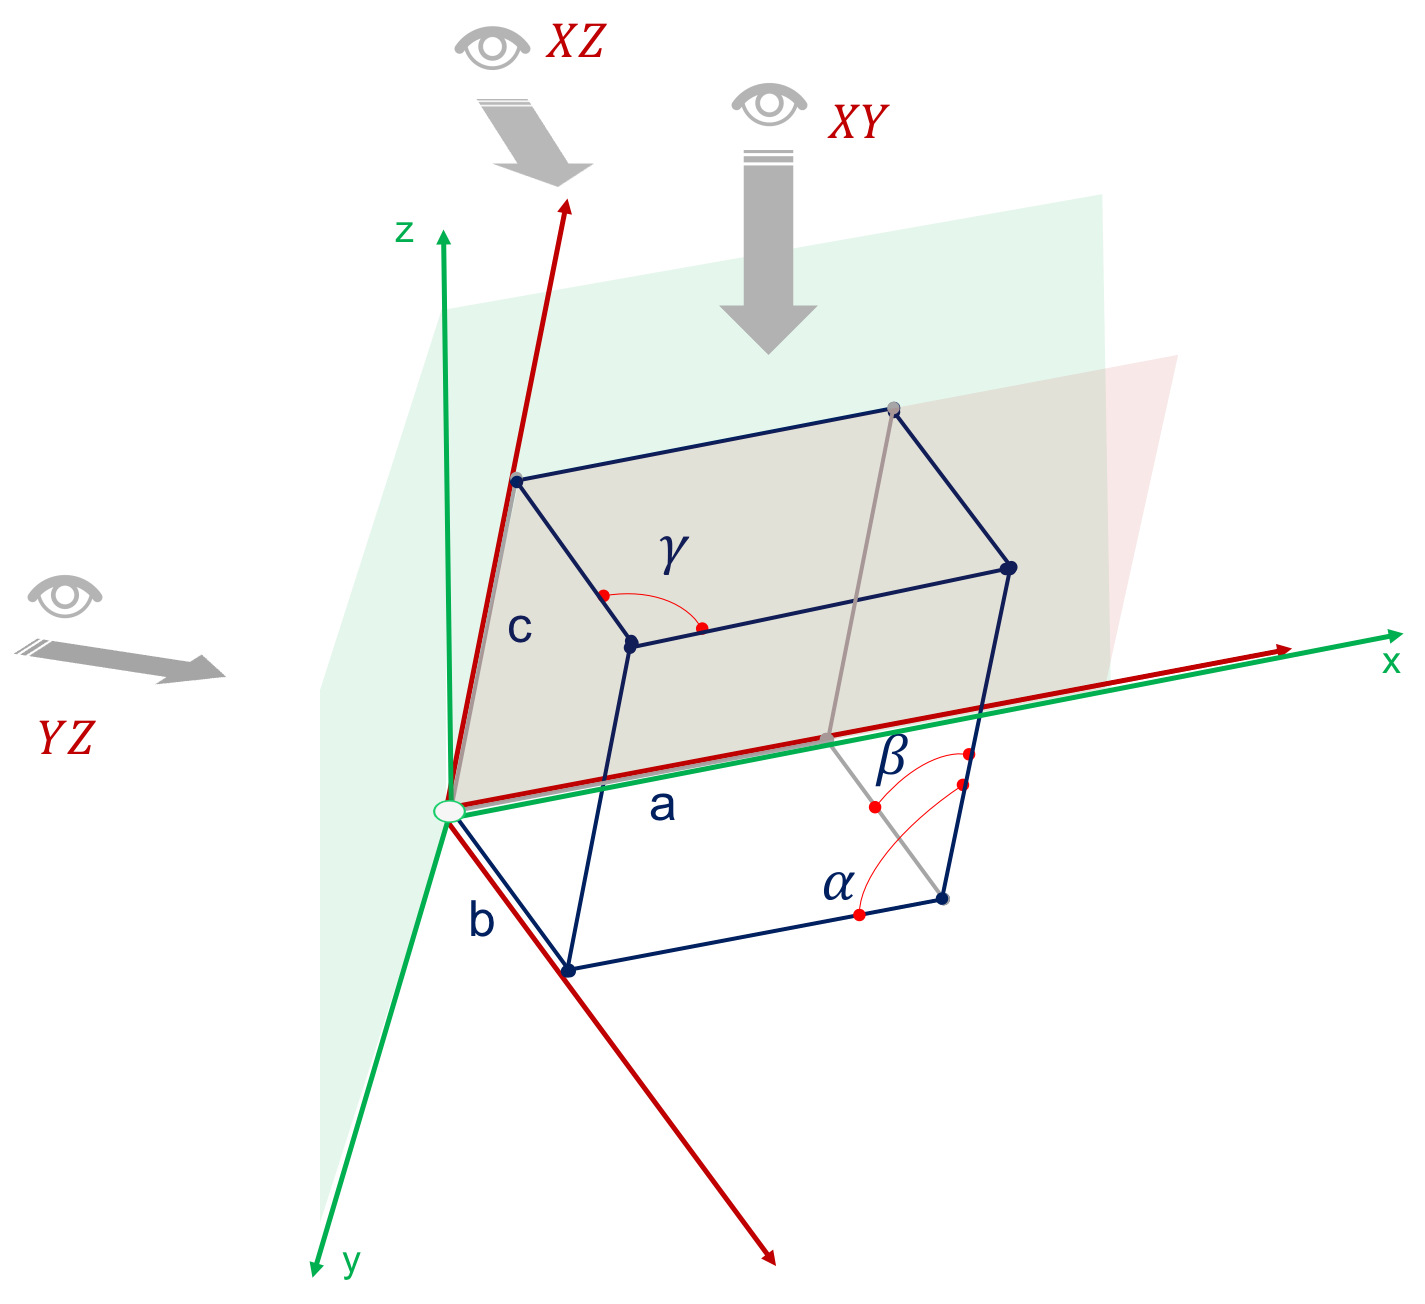
\includegraphics[width=0.59\textwidth]{images/piezo_deformation_general.png}\label{ris:piezo_deformation_general}}
  \hfill
  \subfloat[]{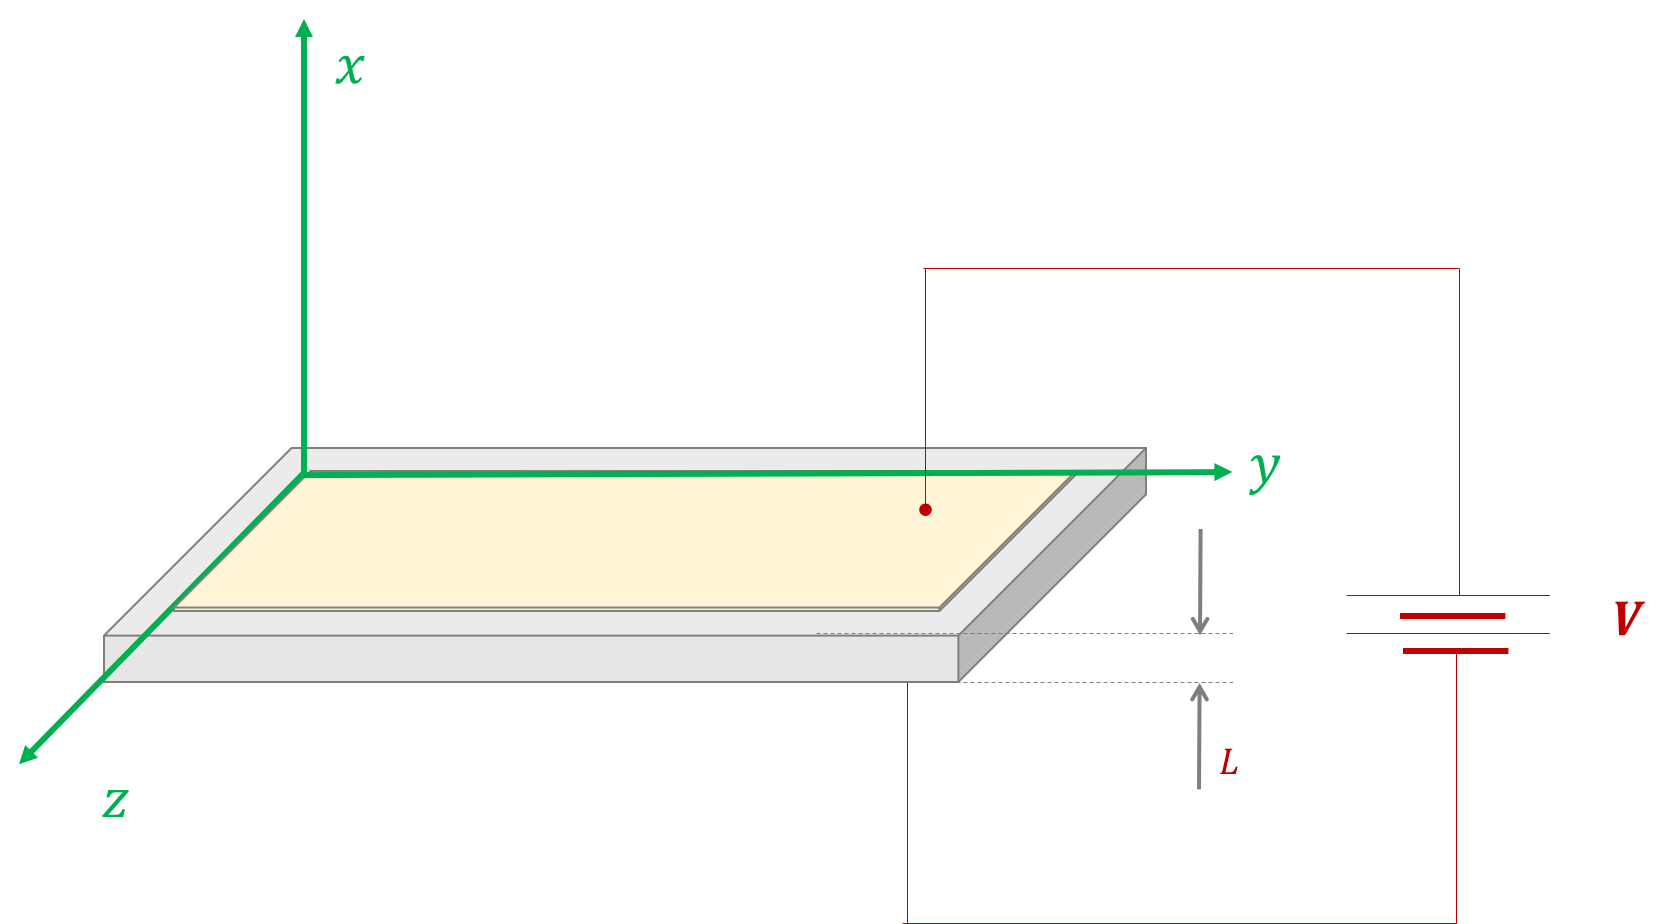
\includegraphics[width=0.39\textwidth]{images/piezo.png}\label{ris:x_cut}}
  \caption{Триклинная ячейка в декартовой система координат (а), x-срез
  кристалла с напыленными на поверхность электродами (b)}
  \label{ris:piezo_deformation_general}
\label{ris:}
\end{figure}


Дальше приведено рассмотрение деформационного поведения элементарной ячейки при работе пьезоэлектрического
эффект в частном случае для кристалла LGT, в котором поле, приложенное вдоль направления X,
вызывает деформации в соответсвии с пьезомодулями $d_{11}$, $d_{12}$ и $d_{14}$ (\ref{sec:piezo_matrix}).

\begin{figure}[H]
  \centering
  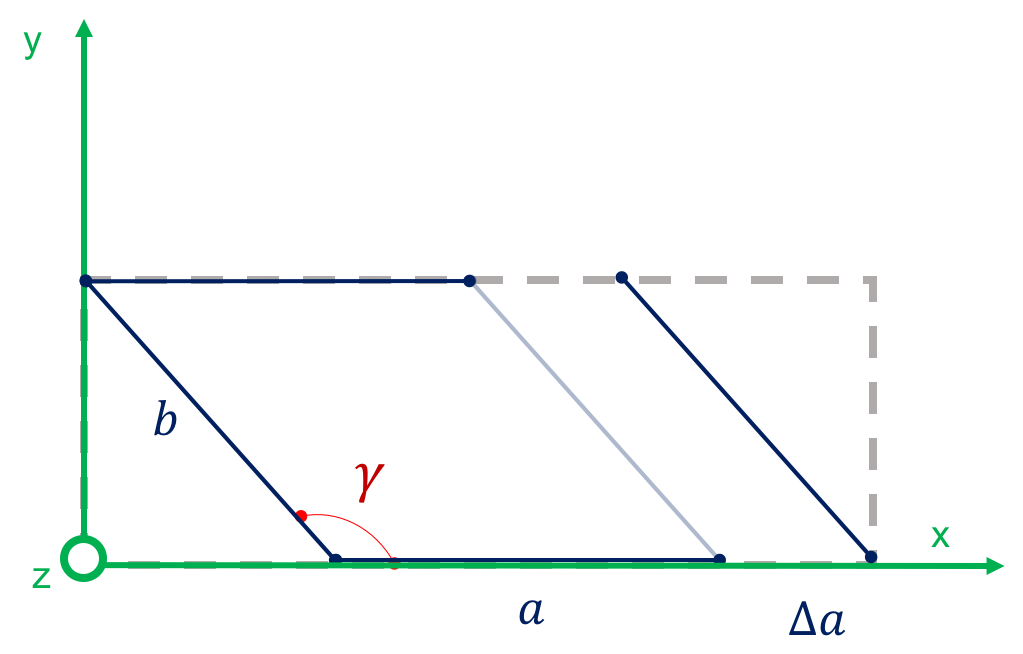
\includegraphics[width=.5\textwidth]{images/d11.png}
  \caption{Схематичное изображение действия пьезомодуля $d_{11}$ на элементарную ячейку LGT}
  \label{ris:d11}
\end{figure}

Пьезомодуль $d_{11}$ характеризуется относительной деформацией растяжения/сжатия $\Delta x/x$, деформация вдоль оси $x$
соответсвует изменению параметра решетки $a$ на величину $\Delta a = d_{11}\cdot a$. %в расчете  на метр/вольт,
Если перпендикулярно оси $x$ вырезать пластинку толщиной $L$
(рис. \ref{ris:x_cut}), и на обкладки такого конденсатора подать напряжение
$V$, то "новый" параметр решетки $a{'}$ будет равен:
\begin{equation}
   a{'}  = a \left(1+\frac{d_{11}\cdot V }{L}\right).
   \label{eq:a_deformed}
\end{equation}

Пьезомодуль $d_{12}$ характеризуется относительной деформацией растяжения/сжатия $dy/y$,
вследствие приложенного электрического поля вдоль направления $x$,
ячейка деформируется по нескольким параметрам одновременно. В таком случае
происходит не только увеличение
параметра $b$, но и изменение угла $\gamma$ (рис. \ref{ris:d12}).

\begin{figure}[H]
  \centering
  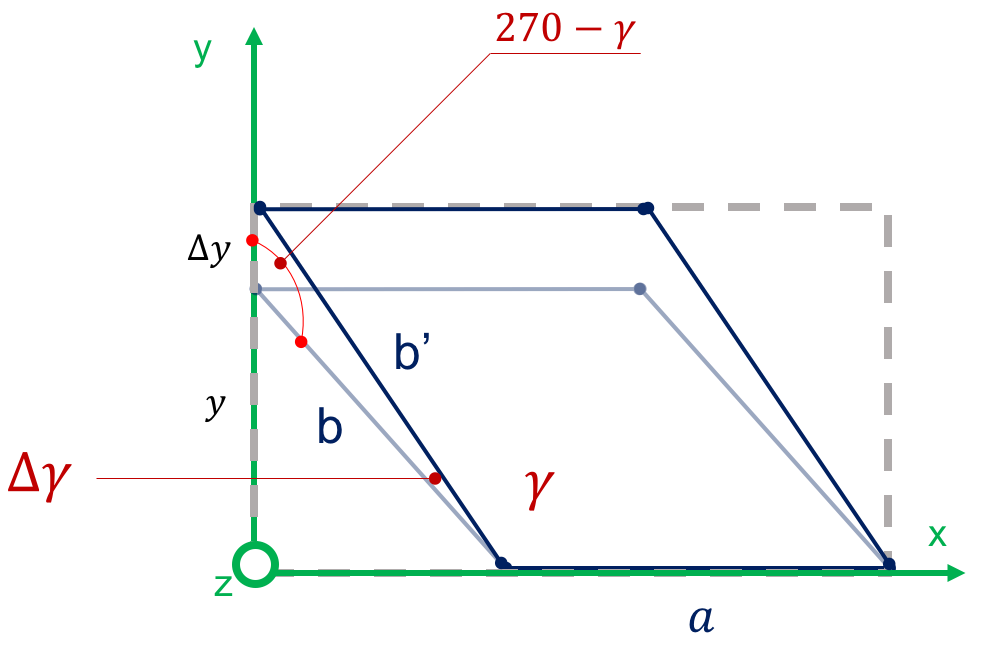
\includegraphics[width=.6\textwidth]{images/d12.png}
  \caption{Вклад пьезоэлектрического модуля $d_{12}$ в деформационное поведение элементарной ячейки, вид сверху ($XY$)}
  \label{ris:d12}
\end{figure}

Исходя из теоремы косинусов измененный параметр $b'$ можно найти по формуле:
\begin{equation}
   b'^2=dy^2+b^2-2 \cdot dy \cdot b \cdot \cos(270-\gamma), \nonumber
   \label{eq:b_formed_1}
\end{equation}
\begin{equation}
   b' = b \sqrt{ 2\sin^2 \gamma \cdot d_{12}+1}.
   \label{eq:b_formed_2}
\end{equation}

Из теоремы синусов выводится измененный параметр $\gamma'$
\begin{equation}
   \frac{\sin(270-\gamma)}{b^{'}} = \frac{\sin (\Delta \gamma)}{dy}, \nonumber
   \label{eq:b_formed_3}
\end{equation}
\begin{equation}
   \gamma^{'} = \gamma + \frac{\cos\gamma \cdot \sin \gamma \cdot d_{12}}{ \sqrt{ \sin^2 \gamma  (d_{12}^2 + 2d_{12})+1}}.
   \label{eq:b_formed_4}
\end{equation}


Сдвиговый пьезомодуль $d_{14}$ характеризует относительную деформацию $dy/z$ и
его действие обуславливается не только
изменением угла $\beta$, но параметром $c$ (рис. \ref{ris:d14}).
\begin{figure}[H]
  \centering
  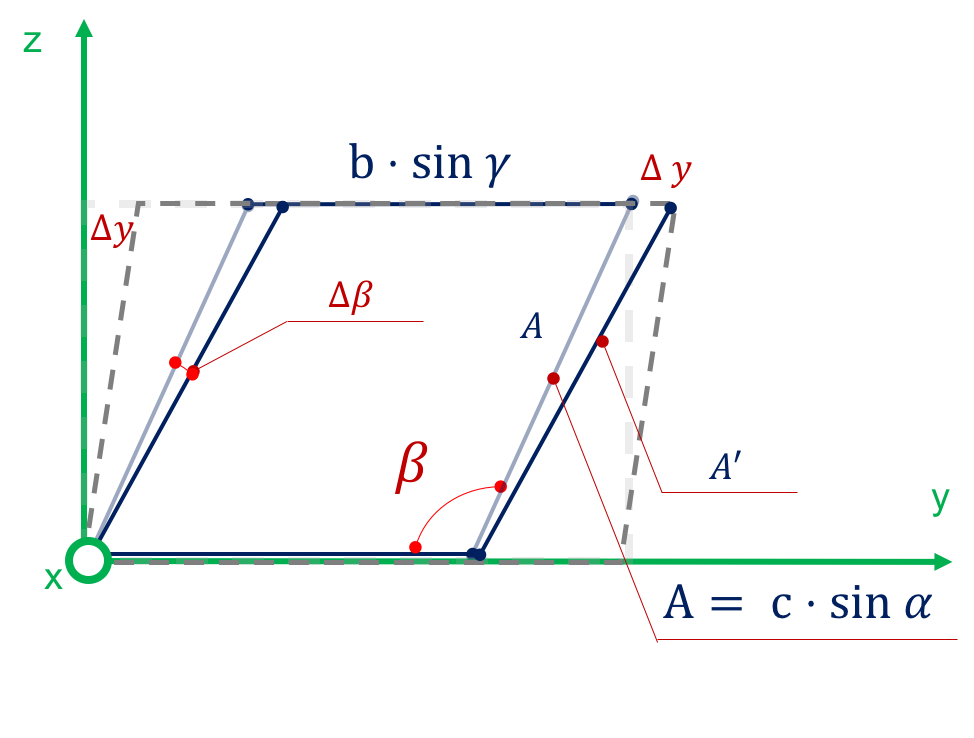
\includegraphics[width=.6\textwidth]{images/d14.png}
  \caption{Схематичное изображение действия модуля $d_{14}$ на деформацию ячейки, вид ($YZ$)}
  \label{ris:d14}
\end{figure}
В соответсвии с теоремой косинусов получим зависимость величины сдвига от параметра решетки $c$,
который находится под наклоном к плоскости $YZ$ на угол $\alpha$ и определяется выражением:
$$
    \Delta y^2 = A^2 + A{'}^2 - 2 A{'}A \cdot \cos \Delta \beta.
$$
В приближении по малому углу $\Delta \beta$ величина сдвига $\Delta y$ будет
определятся разностью длин сторон треугольника
$$
  dy = A^{'} - A.
$$
Из теоремы синусов приращение угла $\beta$ задается выражением,
$$
\Delta \beta = \frac{\Delta y \cdot\sin \beta}{ A+ \Delta y },
$$
\noindent
где
$$
dy = d_{14} \cdot c \cdot \sin \alpha \cdot \sin \beta.
$$
Тогда конечные выражения для измененных под действием модуля $d_{14}$ параметров элементарной ячейки
выглядят следующим образом:
\begin{equation}
   \Delta \beta = \frac{d_{14} \cdot \sin^2\beta}{1+d_{14}\sin \beta},
   \label{eq:b_formed_5}
\end{equation}
\begin{equation}
   c{'} = c(1+d_{14}\sin\beta).
   \label{eq:b_formed_6}
\end{equation}

Для того, чтобы получить значение угла смещения брэгговского максимума,
необходимо рассчитать межплоскостные расстояния соответвующих системе атомных плоскостей
 для выбранных индексов отражения
до (недеформированная ячейка) и после (деформированная) приложения электрического
поля.
